
%%%%%%%%%%%%%%%%%%%%%%% file typeinst.tex %%%%%%%%%%%%%%%%%%%%%%%%%
%
% This is the LaTeX source for the instructions to authors using
% the LaTeX document class 'llncs.cls' for contributions to
% the Lecture Notes in Computer Sciences series.
% http://www.springer.com/lncs       Springer Heidelberg 2006/05/04
%
% It may be used as a template for your own input - copy it
% to a new file with a new name and use it as the basis
% for your article.
%
% NB: the document class 'llncs' has its own and detailed documentation, see
% ftp://ftp.springer.de/data/pubftp/pub/tex/latex/llncs/latex2e/llncsdoc.pdf
%
%%%%%%%%%%%%%%%%%%%%%%%%%%%%%%%%%%%%%%%%%%%%%%%%%%%%%%%%%%%%%%%%%%%

% RECOMMENDED %%%%%%%%%%%%%%%%%%%%%%%%%%%%%%%%%%%%%%%%%%%%%%%%%%%
\documentclass{llncs}
% choose options for [] as required from the list
% in the Reference Guide

\usepackage{mathptmx}       % selects Times Roman as basic font
\usepackage{helvet}         % selects Helvetica as sans-serif font
\usepackage{courier}        % selects Courier as typewriter font
\usepackage{type1cm}        % activate if the above 3 fonts are
                             % not available on your system

\usepackage{makeidx}         % allows index generation
\usepackage{graphicx}        % standard LaTeX graphics tool
                             % when including figure files
\usepackage{multicol}        % used for the two-column index
\usepackage[bottom]{footmisc}% places footnotes at page bottom
\usepackage{amsmath,epsfig}
\usepackage{graphicx}
\usepackage{palatino,epsfig,latexsym}
\usepackage{algorithm}
\usepackage{algorithmic}
\usepackage{amsmath,amsfonts,amssymb,color}
\usepackage{graphicx}
\usepackage{subfigure}
\usepackage{multirow}
\usepackage{bbm}
\usepackage[T1]{fontenc}
\renewcommand{\textfraction}{.01}
\renewcommand{\bottomfraction}{.99}
\renewcommand{\topfraction}{.99}

\usepackage{url}
\newcommand{\keywords}[1]{\par\addvspace\baselineskip
\noindent\keywordname\enspace\ignorespaces#1}
%%%%%%%%%%%%%%%%%%%%%%%%%%%%%%%%%%%%%%%%%%%%%%%%%%%%%%%%%%%%%%%%%%%%%%%%%%%%%%%%%%%%%%%%%

\begin{document}
%\mainmatter  % start of an individual contribution
\title{EvoSpace-Interactive: A Framework to Develop Distributed Collaborative-Interactive Evolutionary Algorithms for Artistic Design}

% a short form should be given in case it is too long for the running head
\titlerunning{EvoSpace-Interactive}


\author{Mario Garc\'ia-Valdez\inst{1} \and Leonardo Trujillo\inst{1}
\and  Francisco Fern\'andez de Vega\inst{2} \and  Juan J. Merelo Guerv\'os\inst{3} \and Gustavo Olague\inst{4}}

\institute{Instituto Tecnol\'ogico de Tijuana, Tijuana BC, Mexico
\and
Grupo de Evoluci\'on Artificial, Universidad de Extremadura, M\'erida, Spain
\and
Universidad de Granada, Granada, Spain
\and
Centro de Investigaci\'on Cient\'ifica y de Educaci\'on Superior de Ensenada,\\ Ensenada BC, Mexico\\
\email{mario@tectijuana.edu.mx,leonardo.trujillo@tectijuana.edu.mx}\\
\email{fcofdez@unex.es,jjmerelo@geneura.ugr.es,olague@cicese.mx}}

\authorrunning{Garc\'ia-Valdez et al.}

% the name(s) of the author(s) follow(s) next
%
% NB: Chinese authors should write their first names(s) in front of
% their surnames. This ensures that the names appear correctly in
% the running heads and the author index.
%
%\author{Alfred Hofmann%
%\thanks{Please note that the LNCS Editorial assumes that all authors have used
%the western naming convention, with given names preceding surnames. This determines
%the structure of the names in the running heads and the author index.}%
%\and Ursula Barth\and Ingrid Haas\and Frank Holzwarth\and\\
%Anna Kramer\and Leonie Kunz\and Christine Rei\ss\and\\
%Nicole Sator\and Erika Siebert-Cole\and Peter Stra\ss er}
%%
%\authorrunning{Lecture Notes in Computer Science: Authors' Instructions}
%% (feature abused for this document to repeat the title also on left hand pages)
%
%% the affiliations are given next; don't give your e-mail address
%% unless you accept that it will be published
%\institute{Springer-Verlag, Computer Science Editorial,\\
%Tiergartenstr. 17, 69121 Heidelberg, Germany\\
%\mailsa\\
%\mailsb\\
%\mailsc\\
%\url{http://www.springer.com/lncs}}
%
%%
%% NB: a more complex sample for affiliations and the mapping to the
%% corresponding authors can be found in the file "llncs.dem"
%% (search for the string "\mainmatter" where a contribution starts).
%% "llncs.dem" accompanies the document class "llncs.cls".
%%
%
%\toctitle{Lecture Notes in Computer Science}
%\tocauthor{Authors' Instructions}
\maketitle


\begin{abstract}
Currently, a large number of computing systems and user applications are focused on distributed and collaborative models for heterogeneous devices, exploiting cloud-based approaches and social networking. However, such systems have not been fully exploited by the evolutionary computation community. This work is an attempt to bridge this gap, and integrate interactive evolutionary computation with a distributed cloud-based approach that integrates with social networking for collaborative design of artistic artifacts. Such an approach to evolutionary art could fully leverage the concept of memes as an idea that spreads from person to person, within a computational system. In particular, this work presents EvoSpace-Interactive, an open source framework for the development of collaborative-interactive evolutionary algorithms, a computational tool that facilitates the development of interactive algorithms for artistic design. A proof of concept application is developed on EvoSpace-Interactive called \emph{Shapes} that incorporates the popular social network Facebook for the collaborative evolution of artistic images generated using the Processing programming language. Initial results are encouraging, \emph{Shapes} illustrates that it is possible to use EvoSpace-Interactive to effectively develop and deploy a collaborative system.
\keywords{Interactive Evolution, Collaborative Design, Evolutionary Art, Cloud Computing}
\end{abstract}


\section{Introduction}
\label{sec:intro}
Evolutionary Algorithms (EAs) where conceived as general techniques capable of addressing a large set of hard optimization problems \cite{DBLP:books/daglib/0015527}.
Yet, their possibilities as a source of creativity were soon devised and applied to art, design and music, to name but a few \cite{ie1}.
Different researchers noticed both, their inherent randomized search process conducting to different solutions
for a single problem when repeatedly running the algorithm,
but also their feasibility when configured to generate novel designs from an aesthetic point of view.
Thus, EAs were soon employed for generating design and art concepts \cite{Bentley:1999:intro}.

Nonetheless, a number of problems has been noticed when dealing with creativity and Evolutionary Algorithms \cite{DBLP:conf/evoW/McCormack05}.
Among them, we can find the difficulties when deciding how to encode design or art concepts within a data structure
-which give rise to individuals and populations-  as well as the definition of useful genetic (search) operators over the chromosome.
A particular hard problem is how to evaluate the quality of individuals within the population when aesthetic concepts are considered.
The problem is that creativity and aesthetic principles are not clearly understood, which keeps from accurately defining a function that can properly  measure it.  Therefore, researchers soon resort to human brains to perform that specific task, thus defining Interactive Evolutionary Algorithms (IEAs):
standard EAs whose fitness evaluations are performed by human beings in an interactive fashion.
Thus, the main loop of the EA includes the human intervention for quality assessment of evolved solutions.
Nevertheless, an inherent drawback arises from the very nature of the model, namely, human fatigue caused by repeated interaction -and some authors have already tried to address this \cite{Frade:2010:EvoGAMES}.
In any case, IEAs have demonstrated their capability for effectively producing art and design \cite{Bentley:1999:intro,Sims:1991,todd:1992}.
We should also mention that typically artists with a strong background in computer science, or computer scientists with art/design interest,
are the researchers involved in this area, since it can be difficult for an artist without programming capabilities to enter this research domain.

Therefore, a disadvantage remains when addressing art and design by means of EAs, when compared with standard optimization problems.
Researchers have developed over the years not only improved versions of the basic operators, models or meta-models for EAs, they have also embedded these
improvements and their algorithms within toolboxes that allow other researchers to easily launch an EA when solving an optimization problem.
This is exactly the opposite for art and design: no EA tool specifically aimed to this field has been design yet.
Researchers have typically implemented specific versions fitted to the problem they try to address,
but no effort is aimed at developing a standard EA-based tool for Art and Design. % La idea es que sea más general? un EA for Art & Design? o ya desde aqui que sea un IEA

Some desirable properties for a specific IEA %  IEA Toolbox?
toolbox useful for artists are:

\begin{enumerate}

	\item An easy process for deploying individuals capable of generative art/design. Given that standard users of this toolboxes will be artists with no background in computer science, an easy means for encoding art concepts should be provided,without the need to understand how to encode an EA;

	\item The direct influences among different artists should not only be allowed, but encouraged, in a collaborative process.

\end{enumerate}

The art world grows on a network of influences that allows ideas to travel between minds.
Authentic memetic  % define memetic and make reference - JJ , creo que se define o aclara en las lineas de abajo -Mario
evolution of artistic ideas arises from an artist's mind and hands, and this should be automatically promoted by a specific toolbox:
memetic evolution without any explicit need of algorithm encoding.
Thus, the term memetic evolution, as originally defined by Richard Dawkins \cite{r.dawkins1976the-selfish-gen}, relying on both minds and computers
would be finally a main component of the evolutionary process.

This work provides the first tool-set that explicitly addresses these issues, a collaborative and interactive EA framework that will easily
allow artists to evolve their creations while interacting
with a network of artists and friends working together around the world.
The remainder of this paper proceeds as follows.
Section \ref{sec:interactive} presents related work on the topic of Interactive Evolution.
Then, Section \ref{sec:evospace} presents the computational platform on which the main proposal of this work is developed.
The proposed collaborative interactive EA is presented in Section \ref{sec:collaborative}.
The experimental work and results are presented in Section \ref{sec:experiments}.
Finally, a concluding remarks are provided in Section \ref{sec:conclusions}.


\section{Related Work}
\label{sec:interactive}
Interactive evolution (IE) incorporates human preferences into the selective pressure that guides the search \cite{ie1,ie2}.
Specifically, IE poses an open-ended evolutionary search, where the objective function of traditional EAs is replaced by a subjective evaluation carried out by a human user of the system.
In one sense, this open-ended nature of IE  broadens the range of feasible solutions that can be reached by the search,
promoting diversity and exploration of design space.
In fact, some of the earliest EAs were open-ended interactive systems, such as the well-known Biomorphs program \cite{biomorphs}.
For instance, IE has been combined with the recently proposed Novelty Search algorithm \cite{ns:2012}, to promote and exploit these properties.

IE is an active area of research, and the approach has been used in a wide variety of applications and problem domains.
However, in this work, emphasis is given to IEAs that were designed to evolve artistic artifacts.
In particular, collaborative systems where many users interact and evaluate an evolving population,
thus guiding the search based on an aggregate of subjective preferences and considerations.
Such systems can be referred to as Collaborative IEAs or C-IEAs.
What follows is not intended as a comprehensive survey, only a review of the most relevant contributions to the present work.


An early example of a web based interactive system is the work by Langdon \cite{langdon:2004}, which evolves fractal representations of virtual creatures.
It proposed a distributed EA using a global population that resides on a central web server and distributes
portions of the population to remote clients using Javascript.
Users evaluate individuals locally and those a user prefers are returned to the server and can be distributed over the web.
Similarly, Secretan et al. \cite{picbreeder} and Clune and Lipson \cite{forms} use web-based IEAs to evolve artistic artifacts
using a generative encoding, compositional pattern producing networks.
Images are evolved in \cite{picbreeder} and 3-D sculptures in \cite{forms} .
In both cases, user (connected clients) collaboration is encouraged.
Both works offer webpages (see Picbreeder.org and EndlessForms.com),
where users can select or create random individuals and evolve lineages of artifacts based on their preferences.
In these systems a user can take a previously evolved artifact and continue the search process himself, building upon a previous evolutionary design in a sequential
manner.
Therefore, evolved artifacts can be the product of a collaborative search process.
Another feature is that evolved artifacts can be rated by users, and since users can create individual accounts, the ratings provide a way to rank users,
or to select previously evolved artifacts based on the particular style of each user.
Furthermore, the collaborative process is captured by the system, since it is possible to visualize how, and when, different users influenced
a genetic lineage.
Kowaliw et al. \cite{evoeco} present another recent example, evolving ecosystemic models, a generative encoding based on multi-agent systems,
that generate high quality artistic drawings.
Users visit a website (\url{http://www.csse.monash.edu.au/~cema/evoeco/}) and interact with a Java applet,
after which they can choose to add evolved images to a central collection,
such that other users can see the resulting images, or use the images as seeds for their own IE design.

The present work builds on previous proposals and extends the C-IEA approach.
First, it promotes collaborative evaluations of artistic artifacts in a dynamic and parallel manner,
instead of the sequential approach followed in \cite{picbreeder,forms}.
Second, it incorporates explicit user interactions by encouraging the use of social networking.
Third, it facilitates the ability to save and share promising artifacts.
Finally, it emphasizes the use of a cloud-based model, with support for multiple computing devices.


\section{EvoSpace}
\label{sec:evospace}
EvoSpace is a population store for the development of evolutionary algorithms that are intended to run on a cloud computing model.
It is designed to be versatile, since the population is decoupled from any particular evolutionary algorithm.
Evospace is asynchronous, client processes, called EvoWorkers, dynamically and asynchronously interact with the EvoSpace store and perform the basic
routines of an evolutionary search.
EvoWorkers can reside on remote clients or on the platform server itself.

EvoSpace consists of two main components.
First, the EvoSpace container that stores the evolving population.
The second component consists of the remote clients called EvoWorkers, which
execute the actual evolutionary process, while EvoSpace is only a population repository.
Figure \ref{fig:evo} illustrates the main components and dataflow within EvoSpace.

\begin{figure*}[t]
    \centering
        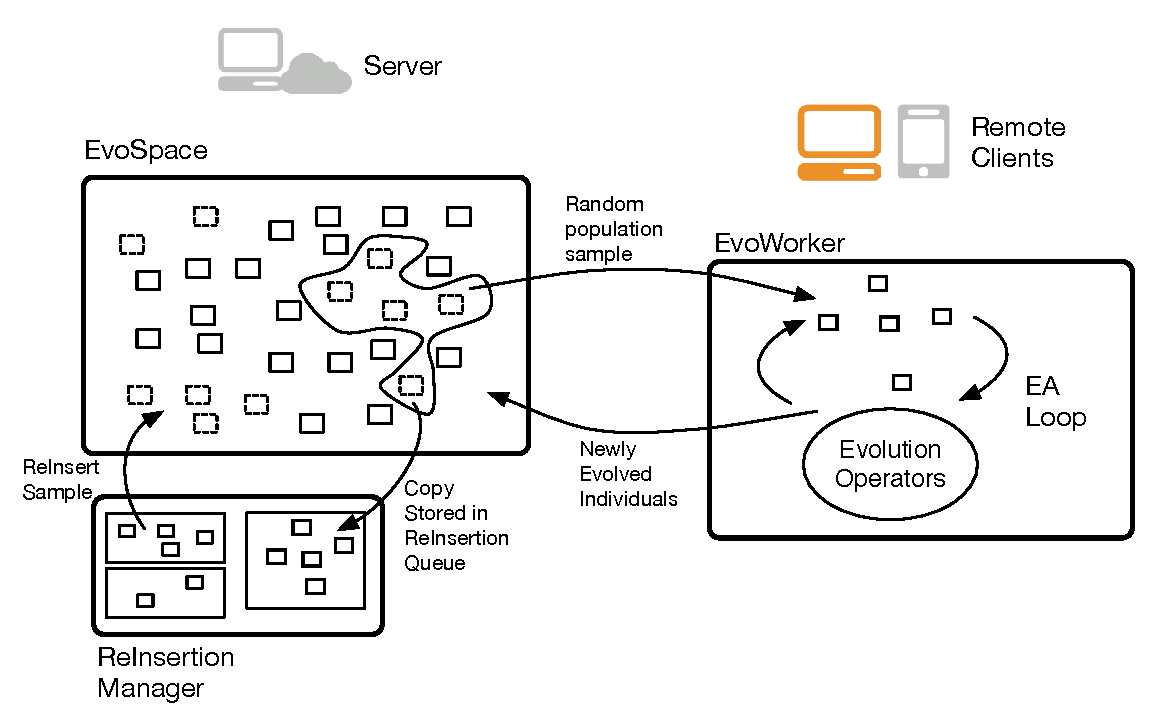
\includegraphics[width=8cm]{evospaceExample.eps}
    \caption{Main components and dataflow within EvoSpace.}
    \label{fig:evo}
\end{figure*}



\subsection{The EvoSpace container.}
EvoSpace is based on the tuplespace model, an associatively addressed memory space shared by several processes.
A tuplespace can be described as a distributed shared memory (DSM) abstraction, organized as a \emph{bag} of tuples.
A tuple $t$ is the basic tuplespace element, composed by one or more fields and corresponding values.
In this model, the basic operations that a process can perform is to insert or withdraw tuples from the tuplespace.
EvoSpace is composed by a set of objects $ES$ and a set of interface methods provided by a central server.
Objects can be withdrawn, processed and replaced into $ES$ using a specified set of methods.
%, while also protecting access rights.
However, EvoSpace is different from other tuplespace implementations in the sense that retrieving and reading objects from ES are random operations.
Individual objects are not of high interest when accessing $ES$, neither is retrieving objects based on search criteria.
Therefore, EvoSpace offers the following interface methods.


\textbf{Read(n):} This method returns a random set $A$ of objects from $ES$, with $|A|=n$ and $A\subset ES$, if $n< |ES|$, the method returns $ES$ otherwise.

\textbf{Take(n):} Returns a random set $A$, following the similar logic used for $Read()$.
However, in this case the sequence of $Take()$ operations provide a temporal dimension to the dynamics of set $ES$.
We can define $ES_i$ as the set at the moment of the $i-th$ $Take()$ operation and $A_i$ as the output.
The contents of EvoSapce are then given by $ES_{i+1}= ES_i \setminus A_i$; i.e., the objets taken are effectively removed from $ES$.
The objects taken are also copied to a new set $S_i$ of \emph{sampled objects} and stored
within a temporary collection $\mathcal{S}$ on the server, implemented as a priority queue.
Sets $S_i \in \mathcal{S}$ can then be reinserted to $ES$ if necessary.

\textbf{ReInsert(i):} This method is used to reinsert the subset of elements removed by the $i-th$ $Take()$ operation,
  such that the contents of EvoSpace are now $ES \cup S_i$ if $S_i \in \mathcal{S}$ and $ES$ is left unchanged otherwise.

\textbf{Insert(A):} This method represents the union operation $ES \cup A$.

\textbf{Replace(A,i):} Similar to $Add()$, however set $A$ should be understood as a replacement for
  some $S_i \in \mathcal{S}$, hence $|A| = |S_i|$, but the objects in $A$ can be different (evolved) objects from those in $S_i$.
  Moreover, if $S_i$ exists it is removed from $\mathcal{S}$.
  However, if $S_i$ does not exist this means that a $ReInsert(i)$ operation preceded it, this increases the size of $ES$.

\textbf{Remove(A):} This method removes all of the objects in $A$ that are also in $ES$, in such a way that
  the contents of EvoSpace are now set to $ES \cup (A\cap ES)$.


\paragraph{Individuals.}
Until now, we have assumed that the objects in $ES$ represent individuals in an EA.
Explicitly, the objects in $ES$ are stored as \emph{dictionaries}, an abstract data type that represents a collection
of unique keys and values, with a one to one association.
In this case, keys represent specific properties of each object and the values can be of different types, such as
numbers, strings, lists, tuples or other dictionaries.


\paragraph{The EvoSpace Server Processes.}
%The EvoSpace architecture employs a client-server architecture with a shared memory container.
On the server side, a process called \texttt{EvoSpaceServer} is executed, which creates and activates a new EvoSpace
container object and waits for requests to execute interface methods.
Additionally, on the server three more processes are executed, these are: \texttt{InitPopulation}, \texttt{ReInsertionMgr} and \texttt{EvolutionMgr}.
\texttt{InitPopulation} is executed once, its goal is initialize the population by adding $popsize$ random
objects. The function that creates new individuals depends on the problem and the representation used.
\texttt{ReInsertionMgr} is used as a failsafe process that periodically checks (every $wt$ seconds) if the size of the population in $ES$
falls below a certain threshold $min$ or if the time after the last reinsetion is greater than $next_r$.
If any of these conditions are satisfied, then $rn$ subsets $S_i \in \mathcal{S}$ are reinserted into ES using the $ReInsertOld()$ method.
%Notice that $ReInsertOld()$ is not an interface method of the EvoSpace shared memory object $ES$, it is an interface provided by the
%EvoSpaceServer, that calls $ReInsert()$ a total of $rn$ times.
Finally, \texttt{EvolutionMgr} periodically checks if a termination condition is satisfied, which is checked by the $isOver()$ method.
This method can be implemented according to the needs of the evolutionary search.
%For instance, $isOver()$ can be used to check if an optimal solution is found or if a maximum number of
%function evaluations have been performed.


\paragraph{EvoSpace Clients: EvoWorkers.}
The \texttt{EvoWorker} process is straightforward, it requests a set of objects $A_i$ from the $ES$ container.
Afterwards, the $Evolve()$ function is called where the actual evolutionary cycle is performed.
In this scenario, $A_i$ can be seen as a local population on which evolution is carried out for $g$ generations.
The result of this evolution is then returned and reinserted into $ES$, afterwards the EvoWorker can request a new set from $ES$ and repeat the process.
Otherwise, each EvoWorker could specialize on a particular part of the evolutionary process, such as selection, evaluation or genetic variation;
an approach not taken in the present paper.


\paragraph{Implementation.}
Individuals are stored in-memory, using the Redis key-value database.
Redis was chosen over a SQL-based management system, or other non-SQL alternatives, because it provides a hash based implementation of sets and queues which are natural data structures for the EvoSpace model. For example, selecting a random key from a set has a complexity of O(1). The logic of EvoSpace is implemented as a Python module exposed as a Web Service using cherrypy and Django HTTP frameworks. The EvoSpace web service can interact with any language supporting json-rpc or ajax requests. The EvoSpace modules and workers in JavaScript, JQuery and python are available with a Simplified BSD License from \url{http://evospace.org}.



\section{A Framework for Collaborative Interactive Evolution}
\label{sec:collaborative}
The goal of this work is to develop an open source framework for Web and Cloud-based C-IEA systems,
using current web standards and libraries for mobile devices.
The framework is called EvoSpace-Interactive, its main components are depicted in Figure \ref{fig:CIE}.
Developers of C-IEA applications are liberated from the need of designing and programming a platform for distributed user collaboration.
Only three components of the framework  must to be defined for each application, marked with double lines in Figure \ref{fig:CIE}; these are:
an \emph{individual} representation; a \emph{processing script} that renders each individual;
and a \emph{worker} script that encodes the evolutionary operators will need to be defined according to the representation and problem domain.
However, in future versions of the framework much of this work could be predefined, but also left open for advanced users to change as they require.
What the framework offers for free is: a central repository for the population implemented as an EvoSpace service; a Web Application script implemented using Django, a mature full stack Web Framework with a BSD license developed in Python.
This application is responsible for user authentication and session handling through the popular Facebook social network using the OAuth 2.0 protocol.
Also, the storage of collections, where users can store individuals they like to share with friends, is persisted using the PostgreSQL DBMS.
Most of the interactive functionality is programmed in the client side using Javascript libraries.
The communication between components is implemented using json-rpc, a lightweight remote procedure call protocol and common ajax and http transactions.
Overall functionality is decomposed in specialized services, adding flexibility to the framework since services can be interchanged.
The framework is build using only open source components from libraries to servers.
Users interact with the system through a GUI implemented on a Responsive Web Design (RWD) front end framework,
an approach to web design in which a graphical user interface is crafted to provide a satisfactory  viewing experience in a range of mobile devices.
This approach will enable designers to tailor the look and feel of the application with minimum intrusion, only changing CSS definitions.
Current functionality from the user perspective is described next.

\begin{figure*}[t]
    \centering
        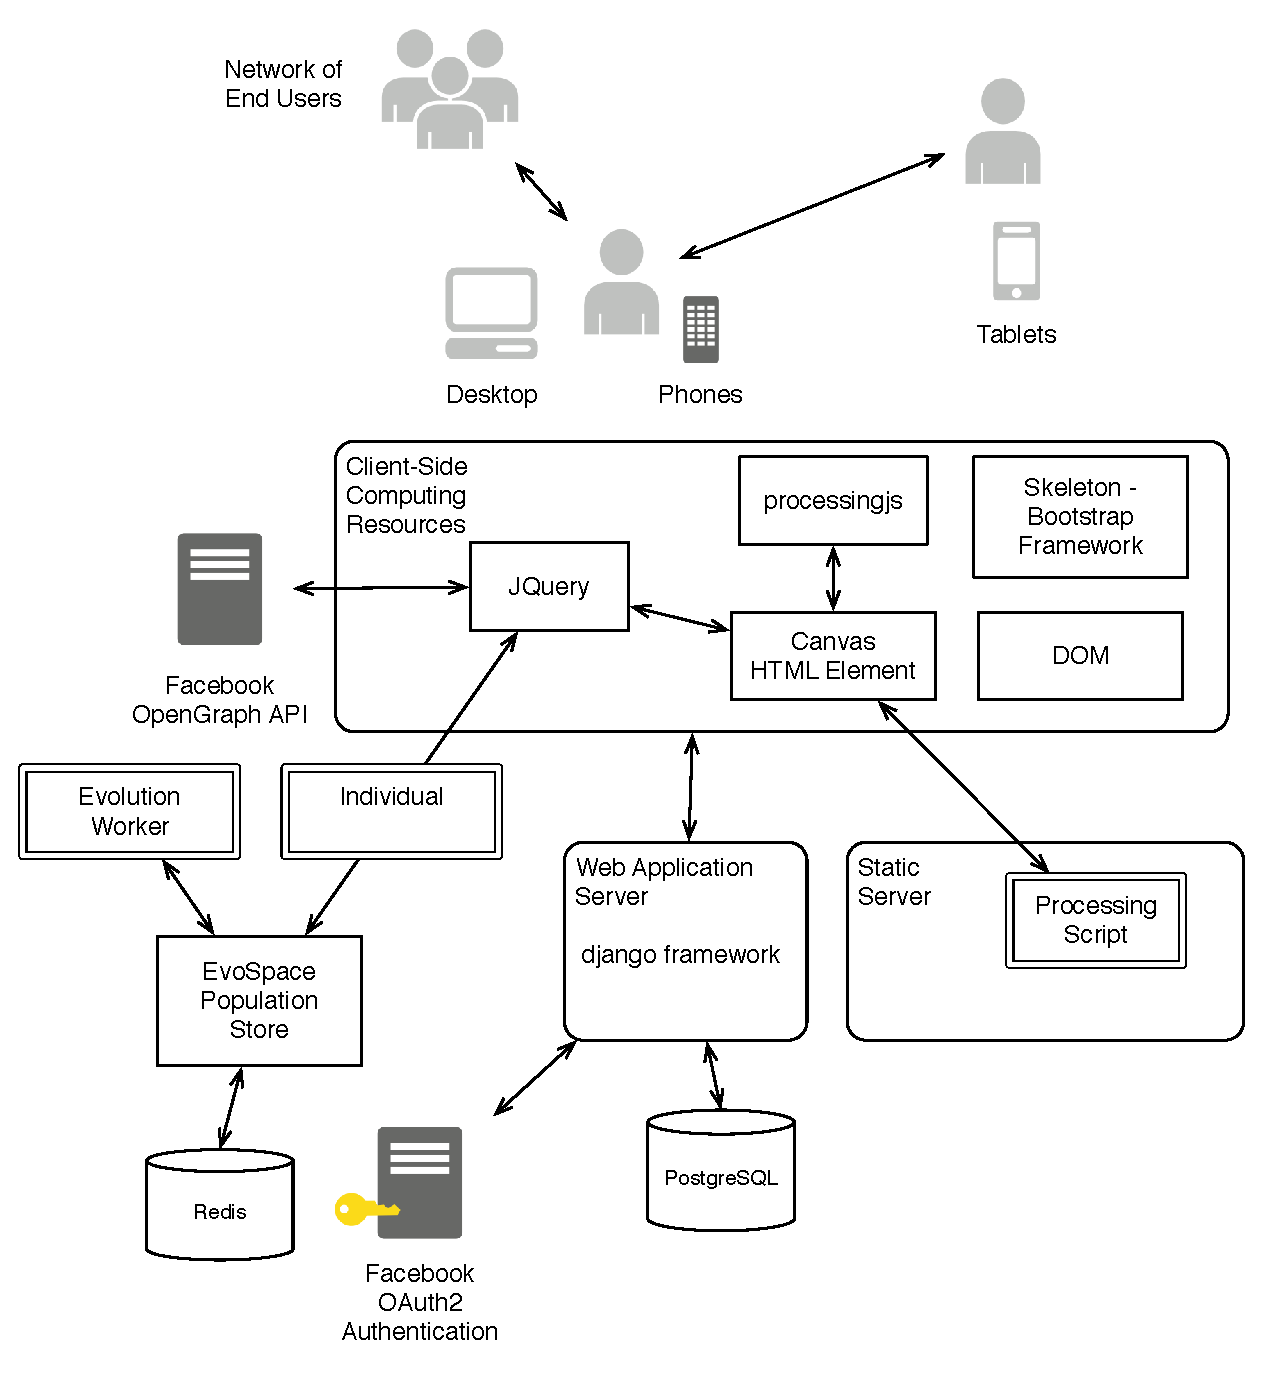
\includegraphics[width=8cm]{arq.eps}
    \caption{Conceptual design of the proposed C-IEA.}
    \label{fig:CIE}
\end{figure*}




\subsection{User Interface}
The users interact with the web interface depicted in Figure \ref{fig:web}, which is composed of five elements.
First, at the top left corner user login and authentication.
Users can login with their Facebook account or participate as anonymous users.
Second, if a user chooses to login a list of Facebook friends that have also linked their account with the C-IEA application is presented on the left,
to encourage users to interact with the system.

\begin{figure*}[t]
    \centering
        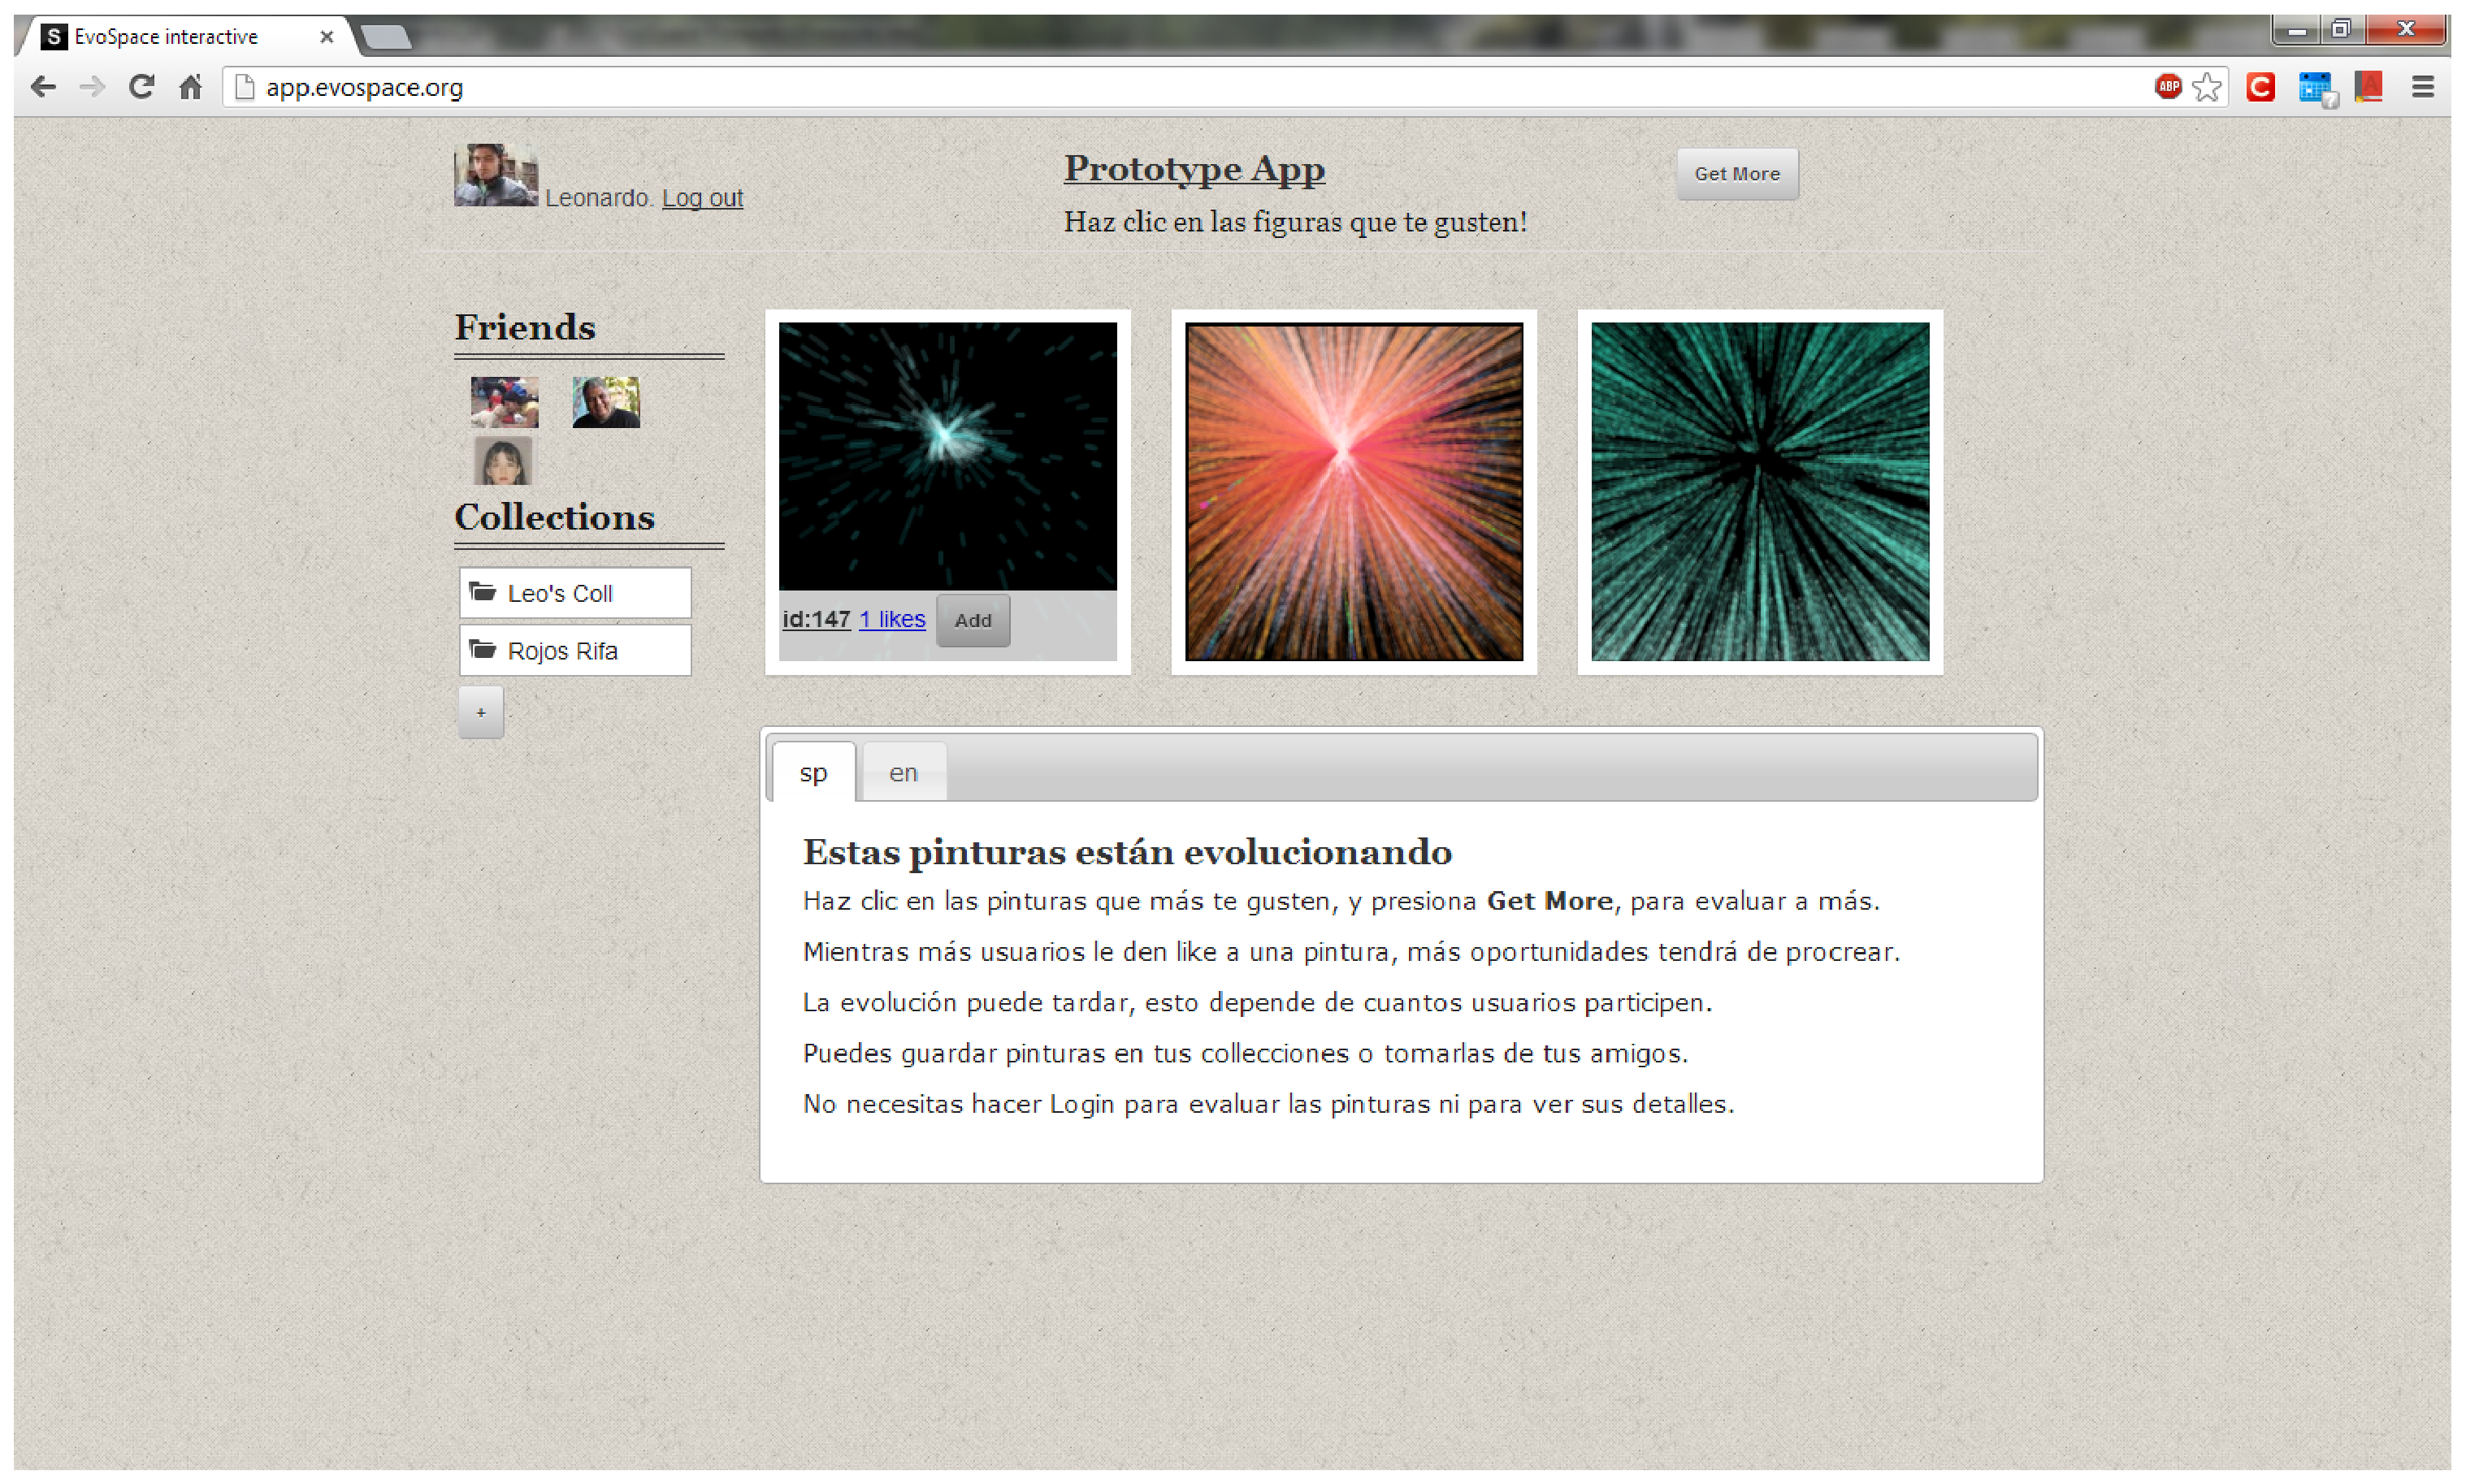
\includegraphics[width=8cm]{EvoApp.eps}
    \caption{User interface of the EvoApp C-IEA.}
    \label{fig:web}
\end{figure*}

The third element is a central \emph{ Wall } area, where a population sample of $n$ individuals is shown to the user.
These are $n$ random individuals taken from the EvoSpace server.
Here, the user can interact with the system in two ways.
He can click on the individuals he prefers, a clicked image is highlighted and this counts as a ''like" for the individual
(this is further explained in the following section).
Additionally, a user can choose to add an image to one of their \emph{Collections}.
A collection is a special directory to store individuals a user prefers and wishes to save.

After the user finishes interacting with the current crop of individuals on the Wall, he can choose to retrieve a new sample from EvoSpace.
This is done with the fourth element of the interface, located at the top of the screen, the \emph{GetMore} button.
The button returns the current group of individuals to EvoSpace, and brings back a new one.
Moreover, each time a user performs a \emph{GetMore} click, it triggers a server-side \emph{Breeding} event,
this event can be used to trigger an application dependent Breeding process.

The fifth element of the interface is shown at the bottom left corner, the \emph{Collections} section.
The user can create several collections, to group and organize his favorite artifacts.
Moreover, a user can browse the content of each collection and from there share images through the social network.
When a user browses over an individual a detail pane shows how many users have liked the individual.
The pane also includes a link to the individual's details, the parents, genetic operators that created it, and genealogy information.

\subsection{Individual Representation}
Individuals are represented internally as a dictionary, as mentioned in Section \ref{sec:evospace}.
The basic properties stored for EvoSapce-Interactive applications are: a unique \texttt{id}; a user defined \texttt{chromosome};
the number of times the individual has been selected in a sample and returned to the population, stored in property called \texttt{views};
the genetic operators that generated the individual; ids of the parents; \texttt{current Fitness} that stores the most resent fitness value;
and a \texttt{fitness} dictionary where each key is a concatenation of a \texttt{userid}, a \texttt{timestamp} and a numerical value that represents
the rating given by the corresponding individual.
A UML representation of an individual is given in Figure \ref{fig:individual}.

%The domain of possible values depends on each implementation, for instance it can be just the number 1 indicating a Like or it could be an integer between 1 and 5 inclusive, to indicate a five star rating. Genetic operators can use the properties stored in each individual's dictionary to calculate the current fitness. Considering for instance each user's experience, a ratio between the number of views and number of likes.

\begin{figure*}[t]
    \centering
        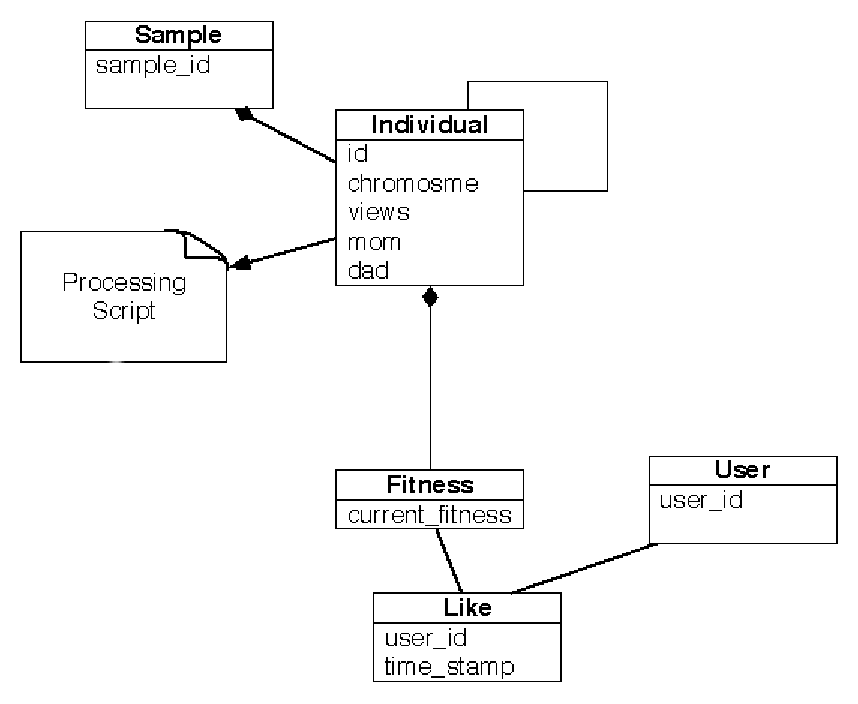
\includegraphics[width=8cm]{UMLIndividual.eps}
    \caption{Individual internal representation }
    \label{fig:individual}
\end{figure*}

\subsection{Processing Language and HTML Canvas Element}
Processing is a programming language and development environment initially created to serve as a software sketchbook and as a tool to teach fundamentals
of computer programming within a visual context.
Currently is used by artists, designers, architects, and researchers for visualization applications, games and interactive animations projects \cite{Reas:2007wp}.
Processing is a subset of Java directed to novice programmers and generative artists \cite{Pearson:2011ti}, which are the intended users of the EvoSpace-Interactive framework.
As a complement there is a javascript library \emph{processingjs} that allows Processing scripts to be run by any HTML5 compatible browser.
Processing scripts are responsible of rendering individuals which can involve animations, sound or even interactive artifacts.
Before calling the \texttt{draw()} method of the processing script initial place holding or fallback parameters are replaced with an individual's chromosome.
Each individual's script has its own Canvas entity, defined by the HTML5 standard as an element that provides scripts with a resolution-dependent bitmap canvas
which can be used for rendering graphics on the fly.
Although the combination of an HTML5 Canvas element and a Processing script is supported by default, other combinations could be used.
For instance, images, embedded audio, or other libraries capable of drawing in the Canvas.
Also, a fallback implementation must be considered for applications intended for non-HTML5 capable browsers.





\section{Experiment: Shapes Application}
\label{sec:experiments}
As a proof of concept a C-EIA application was implemented with the EvoSpace-Interactive framework.
The application is called \emph{Shapes}, and implements each EvoSpace-Interactive component as follows.

\subsection{Individual Representation and Breeding Process}
In \emph{Shapes}, individuals represent a two dimensional 11 by 6 array of equilateral triangles, these arrays are sometimes used in Op-Art style paintings.
Each triangle has a color drawn from a twelve color palette.
The array is represented by a 66 element chromosome vector $\mathbf{v}=(v_1,..v_{66})$, with $v_i \in \{ 1,2,..11 \}$.
The background of the painting is Light Gray, this can give the effect of a missing triangle when it has the same color.
A processing script is used to render a static version of the image.
The breeding process uses tournament selection of size 6 to select two individuals from EvoSpace,
and generates two offspring.
The offspring replace the worst individuals from both tournament groups.
Crossover operators are used with crossover rate of 1, these are vertical and horizontal one-point crossovers.
Several mutations are used with a mutation rate of 0.3, these are:
(1) single \emph{point mutation}; (2) vertical and horizontal \emph{mirrors} at a random point;
(3) \emph{shuffle} that gives a new permutation of the chromosome.



\subsection{Fitness Evaluation}
The fitness of each individual takes into account the evaluation given by several users.
In \emph{Shapes}, users can only give positive evaluations explicitly when they select an individual, a \emph{Like}.
When a user evaluates a sample of individuals, some (or all) of them will not receive a vote, in each case the \texttt{views} property will be incremented by 1.
For instance, if an individual has a high number of views with with only two likes, he is worse than an individual with two views and two likes.
The ratio $Likes/Views$ is more informative, but it does not distinguish between an individual with many views and another with only
one view if they both have zero likes; also views must be >=1 to avoid dividing by zero.
Fitness, therefore, is given by $(Likes+1)/(Views+1)$.

\subsection{System Setup}
The population was initialized with 500 randomly generated individuals. Every second sample returned from users triggers a Breeding process is executed.
\texttt{ES.ReInsert()} method was called when the sample queue reaches a threshold of 20 samples.
A maximum number of concurrent 40 users was expected.
The system was installed in a virtual private server with 500 MB of RAM.
The http Server used was Gunicorn behind a Nginx http proxy.
A simple call for participation was issued by two authors in their personal Facebook and Twitter accounts.
%As a Facebook application, a basic dashboard is freely included where information about user's interactions is presented as \textbf{Insights}.
%A number of graphs are available showing: Number of new users, retention, demographics, traffic, how many users give permission to the application etc.


\subsection{Results}
In nearly two weeks of operation, there is a total of 70 active users, users who gave permissions to the \emph{Shapes} application and haven't
removed it from their Facebook account.
Facebook dashboard reports that 74 percent of users accepted the permission request to use their credentials to login onto \emph{Shapes}.
Participation of anonymous users was permitted, but their number was not recorded.
Basic instructions we're shown in the landing page, but part of the functionality was left to be explored by users.
An auto-increment id was assigned to each individual, after two weeks the highest id number is 8379.
A total of 17449 samples were taken from the EvoSpace server after the two week trial. A sample of artistic artifacts in a collection is depicted in Figure \ref{fig:collection}.
%which shows the genealogical tree that lead to a particular image.

\begin{figure*}[t]
    \centering
        \includegraphics[width=12cm]{collection.eps}
    \caption{Artistic artifacts in a collection }
    \label{fig:collection}
\end{figure*}

\section{Conclusions}
\label{sec:conclusions}
Initial results are encouraging, the EvoSpace-Interactive framework was successfully used to deploy a C-IEA that users accepted and used to design artistic artifacts.
Since the system integrates with a popular social network, the framework promotes the collaborative evolution of artistic memes,
leveraging the insights of multiple users in a parallel and asynchronous manner. The platform enables the collaborative assignment of fitness and provides researchers with relevant contextual information about the process, that can be considered not only in the evaluation step, but also by the system as a whole, allowing a better understanding of user behavior and preferences.
Moreover, through the use of the Processing language, and easy to develop representation of artistic artifacts is possible,
the possibilities of which were not yet pushed to the limit by the simple Shapes application, the main topic of future work and research. Nonetheless, the paper presents the first attempt to build a tool that facilitates the development and deployment of C-IEA for evolutionary art.

\subsubsection*{Acknowledgments.}
\begin{small}
Research supported by DEGEST-ProIFOPEP (Mexico) Research Project 4616.12-P;
CONACYT (Mexico) Basic Science Research Project No. 178323
as well as projects TIN2011-28627-C04-02, TIN2011-28627-C04-02 and -03 (ANYSELF),
awarded by the Spanish Ministry of Science and Innovation, and P08-TIC-03903 awarded by the Andalusian Regional Government also project GRU09105 awarded by Regional Government Junta de Extremadura, Consejería de Economía-Comercio e Innovación and FEDER.
\end{small}

%No hay mucho espacio para conclusiones. Se puede suprimir el gr√°fico
%con la genealogía de un individuo. Por otro lado, "selling points"
% * forma de asignar el fitness
% * Estudio "sociológico" del comportamiento de los usuarios al
% autorizar o no a Facebook (y posible componente viral del mismo si
% se postea en el muro)
% * Naturaliza colaborativa del algoritmo.
%      -Mario  cometarios de JJ?

%\subsubsection*{Aknowledgments}
%This project recived support from DEGEST ProIFOPEP 2012 One year research Grant 2012-2013.

\bibliographystyle{abbrv}
\begin{footnotesize}
\bibliography{biblio}
\end{footnotesize}

\end{document} 